%% LyX 2.3.6.1 created this file.  For more info, see http://www.lyx.org/.
%% Do not edit unless you really know what you are doing.
\documentclass[english]{article}
\usepackage[T1]{fontenc}
\usepackage[latin9]{inputenc}
\usepackage{geometry}
\geometry{verbose,tmargin=2.5cm,bmargin=2.5cm,lmargin=2.5cm,rmargin=2.5cm}
\usepackage{color}
\usepackage{calc}
\usepackage{textcomp}
\usepackage{graphicx}

\makeatletter

%%%%%%%%%%%%%%%%%%%%%%%%%%%%%% LyX specific LaTeX commands.
%% Because html converters don't know tabularnewline
\providecommand{\tabularnewline}{\\}

\makeatother

\usepackage{babel}
\begin{document}
{[}SPLIT\_HERE{]}
\begin{enumerate}
\item \textbf{{[}ALVL/9597/2013/P1/Q1{]} }

The files \texttt{WORDS1.TXT} and \texttt{WORDS2.TXT} store a list
of single word computing terms used in a textbook.

Each entry has the following format: 

\texttt{<computing term>}

\texttt{<number>}

One of the file entries (in both files) is:

\texttt{program }

\texttt{52}

This means that after a complete scan of the textbook the word 'program'
was found 52 times.

\subsubsection*{Task 1.1}

Write program code to find and output the term with the highest number
of occurrences. Use the file \texttt{WORDS1.TXT} to test your program.

\subsubsection*{Evidence 1}

The program code. \hfill{}{[}8{]}

\subsubsection*{Evidence 2}

Screenshot of output. \hfill{}{[}1{]}

\subsubsection*{Task 1.2}

Amend your program code so that if more than one term exists with
the highest number of occurrences, all terms are reported. Use the
file \texttt{WORDS2.TXT} to test your program.

\subsubsection*{Evidence 3}

The program code. \hfill{}{[}5{]}

\subsubsection*{Evidence 4}

Screenshot of output.\hfill{} {[}1{]}

{[}SPLIT\_HERE{]}

\quad{}
\item \textbf{{[}ALVL/9597/2013/P1/Q2{]} }

A company keeps data about its employees. The employee surname and
employee ID are recorded. 

All employee IDs are unique and have the format C999 where C is any
uppercase letter and 9 is a digit.

A program is to be produced to search by either:
\begin{itemize}
\item The surname, which then reports the matching employee ID
\item The employee ID, which then reports the matching surname
\end{itemize}
The programmer stores the data a two 1-dimensional arrays and produces
the following search algorithm to search a string array and output
the matching value from the second array.

\noindent %
\noindent\begin{minipage}[t]{1\columnwidth}%
\texttt{INPUT SearchItem }

\texttt{FOR Index \textleftarrow{} 1 TO UpperBound }

\texttt{\qquad{}IF SearchItem = Array1{[}Index{]} }

\texttt{\qquad{}\qquad{}THEN OUTPUT Array2{[}Index{]} }

\texttt{\qquad{}ENDIF }

\texttt{ENDFOR}%
\end{minipage}

This search algorithm is inefficient.

The programmer uses the following design to produce the program code:
\begin{itemize}
\item code to search by surname 
\item The search algorithm has \texttt{Surname} as \texttt{Array1} and \texttt{EmployeeID}
as \texttt{Array2} followed by code to search by employee ID 
\item The search algorithm has \texttt{EmployeeID} as \texttt{Array1} and
\texttt{Surname} as \texttt{Array2}
\end{itemize}
This design would produce repetition of code.

\subsubsection*{Task 2.1}

Write program code which performs each of the searches:
\begin{itemize}
\item Search by surname 
\item Search by employee ID
\end{itemize}
Your code should address the issues of inefficiency and repetition
of code described in the scenario above. 

Use the sample array data available from the text file \texttt{EMPLOYEEDATA.txt}
and paste this into your program code.

\subsubsection*{Evidence 5}

Your program code.\hfill{} {[}11{]}

\subsubsection*{Task 2.2}

Devise a set of four test cases with the data to be used.

\subsubsection*{Evidence 6}

A screenshot for each test case you considered. Annotate the screenshot
explaining the purpose of each test. \hfill{}{[}4{]}

{[}SPLIT\_HERE{]}

\quad{}
\item \textbf{{[}ALVL/9597/2013/P1/Q3{]} }

The task is to store a dataset (maximum size 20 items) as a binary
tree structure. You should assume that the data items are unique.

The program will use a user-defined type Node for each node defined
as follows:
\begin{center}
\begin{tabular}{|l|l|l|}
\hline 
\texttt{\hspace{0.01\columnwidth}}Identifier & \texttt{\hspace{0.01\columnwidth}}Data Type & \texttt{\hspace{0.05\columnwidth}}Description\tabularnewline
\hline 
\texttt{LeftP} & \texttt{INTEGER} & The left pointer for the node\tabularnewline
\hline 
\texttt{Data} & \texttt{STRING} & The node's data value\tabularnewline
\hline 
\texttt{RightP} & \texttt{INTEGER } & The right pointer for the node\tabularnewline
\hline 
\end{tabular}
\par\end{center}

A linked list is maintained of all the unused nodes which do not form
part of the tree. The first available node which is used for a new
term is indicated by NextFreePosition. Items in the unused list are
linked using their left pointers.

The binary tree and linked list are implemented using variables as
follows:
\begin{center}
\begin{tabular}{|l|l|l|}
\hline 
\texttt{\hspace{0.01\columnwidth}}Identifier & \texttt{\hspace{0.01\columnwidth}}Data Type & \texttt{\hspace{0.05\columnwidth}}Description\tabularnewline
\hline 
\texttt{ThisTree} & \texttt{ARRAY{[}20{]} : Node} & The tree data\tabularnewline
\hline 
\texttt{Root } & \texttt{INTEGER} & Index for the root position of the \texttt{ThisTree} array\tabularnewline
\hline 
\texttt{NextFreePosition} & \texttt{INTEGER } & Index for the next unused node\tabularnewline
\hline 
\end{tabular}
\par\end{center}

\begin{center}
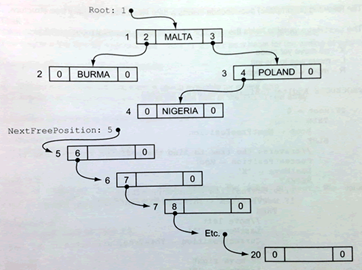
\includegraphics[width=0.5\paperwidth]{C:/Users/Admin/Desktop/Github/question_bank/LyX/static/img/9597-ALVL-2013-P1-Q3}
\par\end{center}

The diagram shows the binary tree and linked list after four values
have been added.

\subsubsection*{Task 3.1}

Write the program code to declare all the required variables and create
the initial linked list which contains all 20 nodes. Add statement(s)
to initialise the empty tree.

\hfill{}{[}10{]}

\subsubsection*{Evidence 7}

Your program code for Task 3.1. {[}11{]}

The following (incomplete) pseudocode inserts a data value into the
binary tree structure.

The \texttt{LastMove} variable holds the direction of the previous
traversal move as follows:

X - no move yet made 

L - move was to the left 

R - move was to the right

\noindent %
\noindent\begin{minipage}[t]{1\columnwidth}%
\texttt{PROCEDURE AddItemToBinaryTree(NewFreeItem)}

\texttt{\qquad{}IF Root = 0}

\texttt{\qquad{}\qquad{}THEN}

\texttt{\qquad{}\qquad{}\qquad{}Root \textleftarrow{} NextFreePosition}

\texttt{\qquad{}\qquad{}ELSE}

\texttt{\qquad{}\qquad{}\qquad{}// traverse the tree to find the
position for the new value}

\texttt{\qquad{}\qquad{}\qquad{}CurrentPosition \textleftarrow{}
Root}

\texttt{\qquad{}\qquad{}\qquad{}LastMove \textleftarrow{} 'X'}

\texttt{\qquad{}\qquad{}\qquad{}REPEAT}

\texttt{\qquad{}\qquad{}\qquad{}\qquad{}PreviousPosition \textleftarrow{}
CurrentPosition}

\texttt{\qquad{}\qquad{}\qquad{}\qquad{}IF NewFreeItem < ThisTree{[}CurrentPosition{]}.Data}

\texttt{\qquad{}\qquad{}\qquad{}\qquad{}\qquad{}THEN}

\texttt{\qquad{}\qquad{}\qquad{}\qquad{}\qquad{}\qquad{}// move
left}

\texttt{\qquad{}\qquad{}\qquad{}\qquad{}\qquad{}\qquad{}LastMove
\textleftarrow{} 'L'}

\texttt{\qquad{}\qquad{}\qquad{}\qquad{}\qquad{}\qquad{}CurrentPosition
\textleftarrow{} ThisTree{[}CurrentPosition{]}.LeftP}

\texttt{\qquad{}\qquad{}\qquad{}\qquad{}\qquad{}ELSE}

\texttt{\qquad{}\qquad{}\qquad{}\qquad{}\qquad{}\qquad{}// move
right}

\texttt{\qquad{}\qquad{}\qquad{}\qquad{}\qquad{}\qquad{}LastMove
\textleftarrow{} 'R'}

\texttt{\qquad{}\qquad{}\qquad{}\qquad{}\qquad{}\qquad{}CurrentPosition
\textleftarrow{} ThisTree{[}CurrentPosition{]}.RightP}

\texttt{\qquad{}\qquad{}\qquad{}\qquad{}ENDIF}

\texttt{\qquad{}\qquad{}\qquad{}UNTIL CurrentPosition = 0}

\texttt{\qquad{}ENDIF}

\texttt{\qquad{}IF LastMove = 'R'}

\texttt{\qquad{}\qquad{}THEN}

\texttt{\qquad{}\qquad{}\qquad{}ThisTree{[}PreviousPosition{]}.RightP
\textleftarrow{} NextFreePosition}

\texttt{\qquad{}\qquad{}ELSE}

\texttt{\qquad{}\qquad{}\qquad{}ThisTree{[}PreviousPosition{]}.LeftP
\textleftarrow{} NextFreePosition}

\texttt{\qquad{}ENDIF}

\texttt{\qquad{}NextFreePosition ThisTree{[}NextFreePosition{]}.LeftP}

\texttt{ENDPROCEDURE}%
\end{minipage}

Note: The above text is available in the text file \texttt{PSEUDOCODE\_TASK\_3\_2.TXT}

\subsubsection*{Task 3.2}

Write non-recursive code to implement the \texttt{AddItemToBinaryTree}
procedure. You may use the text file \texttt{PSEUDOCODE\_TASK\_3\_2.TXT}
as a basis for the writing of your code.

The given pseudocode is incomplete as:
\begin{itemize}
\item it does not initially test that there is space available for a new
item 
\item it does not assign \texttt{NewTreeItem} to the data field of the \texttt{ThisTree}
array
\end{itemize}
Add these requirements to your program solution.

\subsubsection*{Evidence 8}

Your program code for Task 3.2.\hfill{} {[}6{]}

\subsubsection*{Task 3.3}

Write a procedure\texttt{ OutputData} which displays the value of
\texttt{Root}, the value of \texttt{NextFreePosition} and the contents
of \texttt{ThisTree} in index order.

\subsubsection*{Evidence 9}

Your program code for Task 3.3. \hfill{}{[}5{]}

\subsubsection*{Task 3.4}

Write a main program to:
\begin{itemize}
\item Input new data items and add them to the binary tree by calling procedure
\texttt{AddItemToBinaryTree}. The input is terminated with value \textquotedbl\texttt{XXX}\textquotedbl .
Do not attempt to validate the input of the country names. 
\item Your program will then call procedure \texttt{OutputData}.
\end{itemize}
Run the program with the input of the single value \textquotedbl\texttt{XXX}\textquotedbl .

\subsubsection*{Evidence 10}

Screenshot showing the output from running the program in Task 3.4.\hfill{}
{[}3{]}

\subsubsection*{Task 3.5}

Test your program using the following data items input in the order
shown:
\begin{center}
\texttt{INDIA, NEPAL, MALAYSIA, SINGAPORE, BURMA, CANADA, LATVIA,
XXX}
\par\end{center}

\subsubsection*{Evidence 11}

Provide screenshot test evidence for Task 3.5. \hfill{}{[}5{]}

Further program code is required to carry out an \textbf{in-order
traversal}.

\subsubsection*{Task 3.6}

Write a recursive procedure to carry out an in-order tree traversal. 

Include a call to the procedure from your main program.

\subsubsection*{Evidence 12}

Your program code. \hfill{}{[}8{]}

\subsubsection*{Evidence 13}

Produce a screenshot for the Task 3.5 dataset confirming the output
of the countries in alphabetical order. \hfill{}{[}2{]}

{[}SPLIT\_HERE{]}

\quad{}
\item \textbf{{[}ALVL/9597/2013/P1/Q4{]} }

The task is to input data for a frequency distribution and then output
to the screen a horizontal bar chart.

The data is input as an X value followed by its frequency. Assume
the frequency is always in the range 0 to 60 and there are no more
than six X values.

The input shown below shows the number of sweatshirts sold in a retail
shop over a one week period; for example there were 39 XL items sold

\noindent\fbox{\begin{minipage}[t]{1\columnwidth - 2\fboxsep - 2\fboxrule}%
\texttt{Next X value ... <ZZZ to END> XS }

\texttt{Frequency ... 12 }

\texttt{Next X value ... <ZZZ to END> S }

\texttt{Frequency ... 22 }

\texttt{Next X value ... <ZZZ to END> M }

\texttt{Frequency ... 45 }

\texttt{Next X value ... <ZZZ to END> L }

\texttt{Frequency ... 56 }

\texttt{Next X value ... <ZZZ to END> XL }

\texttt{Frequency ... 39 }

\texttt{Next X value ... <ZZZ to END> XXL}

\texttt{Frequency ... 11 }

\texttt{Next X value ... <ZZZ to END> ZZZ}

\texttt{++++++++++++++++++++++++++++++++++++++++}

\texttt{Frequency distribution }

\texttt{++++++++++++++++++++++++++++++++++++++++}

\texttt{XS ~@@@@@@@@@@@@ }

\texttt{S ~~@@@@@@@@@@@@@@@@@@@@@@ }

\texttt{M ~~@@@@@@@@@@@@@@@@@@@@@@@@@@@@@@@@@@@@@@@@@@@@@ }

\texttt{L ~~@@@@@@@@@@@@@@@@@@@@@@@@@@@@@@@@@@@@@@@@@@@@@@@@@@@@@@@@ }

\texttt{XL ~@@@@@@@@@@@@@@@@@@@@@@@@@@@@@@@@@@@@@@@ }

\texttt{XXL @@@@@@@@@@@}%
\end{minipage}}

\subsubsection*{Task 4.1}

Write a program which inputs a set of X values and frequencies and
produces output in the format shown.

\subsubsection*{Evidence 14}

Your program code for Task 4.1.\hfill{}{[}8{]}

\subsubsection*{Evidence 15}

A screenshot to confirm the dataset used and the output produced.
\hfill{}{[}2{]}

The appearance of the bar chart display is to be improved as follows:
\begin{itemize}
\item Each bar is to be represented by more than one line of the same character
to that its bar width is increased. 
\item Each bar will be shown with the same number of lines. 
\item The complete bar chart, including the heading, is to take up no more
than 40 lines. 
\item The line width for the output is exactly 80 characters. 
\item Its appearance could be improved by changing the @ character.
\end{itemize}

\subsubsection*{Task 4.2}

Write code to produce a new chart for the data used in Task 4.1 showing
the maximum possible bar width and any other refinements you have
introduced.

\subsubsection*{Evidence 16}

Your program code for Task 4.2. \hfill{}{[}4{]}

\subsubsection*{Evidence 17}

A screenshot showing the data entry followed by the bar chart. \hfill{}{[}2{]}

Some datasets will have a frequency which is greater than 60 and so
the frequencies of the dataset can no longer be shown with a corresponding
number of characters in the line. The frequencies will need to be
scaled before the output is attempted.

The bar chart would benefit by the inclusion of a horizontal axis
labelled with a scale showing the frequency values.

\subsubsection*{Task 4.3}

Revise your program code to meet these new requirements.

\subsubsection*{Evidence 18}

Your program code for Task 4.3.\hfill{} {[}8{]}

\subsubsection*{Evidence 19}

Screenshots demonstrating: 
\begin{itemize}
\item Dataset 1 as used in Task 4.1 which needs no scaling 
\item Dataset 2 of your choice to demonstrate frequencies which must be
scaled 
\item Dataset 3 of your choice to demonstrate frequencies which must be
scaled differently to Dataset 2 
\end{itemize}
\hfill{}{[}6{]}

{[}SPLIT\_HERE{]}
\item \textbf{{[}ALVL/9597/2013/P2/Q1{]} }

A dental practice currently uses a computer system to store details
of its patients, staff and appointments in separate files.

The practice manager and the receptionist have their own computers
for accessing and updating the files.

The system produces a small number of reports.

An updated system is to be produced by a software company. The updated
system will use a database. In the updated system the dentists will
be given a hand-held device to use in their rooms for accessing and
updating the patient records. The new system will also be capable
of producing additional reports.

The software company has software engineers who have expert skills
in specific areas of software development. A number of the engineers
will be involved in the development of the updated system.
\begin{enumerate}
\item Describe and justify three methods which can be used to determine
what further reports are required from the updated computer system.
{[}6{]}
\item The work to update the system is partly managed by the following Program
Evaluation and Review Technique (PERT) chart.

A - investigation 

B - analysis 

C - design of database 

D - design of reports 

E - design of screen displays for dentists 

F - transfer of data from files into database 

G - documentation produced 

H - acceptance testing 

I - hand over to customer

Time is measured in weeks.
\begin{center}
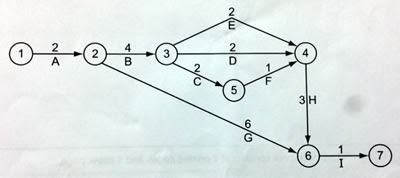
\includegraphics[width=0.5\paperwidth]{C:/Users/Admin/Desktop/Github/question_bank/LyX/static/img/9597-ALVL-2013-P2-Q1-1}
\par\end{center}
\begin{enumerate}
\item State the critical path.\hfill{} {[}1{]}
\item State the minimum time in which the updated system could be operational.
\hfill{}{[}1{]}
\item For activity E state the 
\begin{itemize}
\item earliest Start time 
\item earliest Finish time 
\item latest Start time
\item latest Finish time\hfill{}{[}4{]}
\end{itemize}
\end{enumerate}
\item {}\textcolor{white}{\_}
\begin{center}
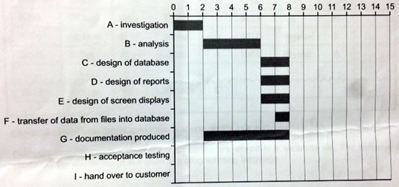
\includegraphics[width=0.5\paperwidth]{C:/Users/Admin/Desktop/Github/question_bank/LyX/static/img/9597-ALVL-2013-P2-Q1-2}
\par\end{center}

The Gantt chart above is based on the information in part \textbf{(b)}.
The timing of two activities is missing and also the timing of one
of the activities shown is incorrect.

Draw a sketch of the Gantt chart to show the correct version. \hfill{}{[}4{]}
\item Explain how the Gantt chart can help with the work that the software
engineers have to carry out. \hfill{}{[}2{]}
\item A small team is put together to consider security aspects of the updated
system.
\begin{enumerate}
\item Identify \textbf{two} possible members of the team and justify your
choice.\hfill{} {[}4{]}
\end{enumerate}
The team have to produce a report to which they all make a contribution.
The report is stored on a network. Each member of the team has access
to allow them to add their contribution.
\begin{enumerate}
\item[ii]  Give \textbf{two} examples of unethical behaviour by a team member.\hfill{}
{[}2{]}
\end{enumerate}
\item Name and describe \textbf{two} types of documentation produced for
this project.\hfill{} {[}6{]}

\noindent\fbox{\begin{minipage}[t]{1\columnwidth - 2\fboxsep - 2\fboxrule}%
End-User documentation 
\begin{itemize}
\item for actual users of system to learn about features and how to use
them 
\item minimum/recommended hardware and software system requirements (operating
system, version, processor, amount of RAM and hard disk space, etc.) 
\item installation guide + step by step guide of how to perform a task or
use a feature 
\item frequently asked questions (FAQ) for common troubleshooting problems
and solutions 
\item support contact information, safety instructions, warranty information
\end{itemize}
Technical documentation
\begin{itemize}
\item for developers to document technical requirements and features of
system
\item system objectives and scope 
\item input and output/report specifications 
\item data storage/database specification 
\item modules/processes and algorithms 
\item user interfaces and application programming interfaces (APIs) 
\item testing
\item implementation/deployment 
\item bugs report and known issues
\end{itemize}
%
\end{minipage}}
\end{enumerate}
The hand-held devices the dentists use in their practice rooms will
be networked. Both client-side scripting and server-side scripting
will be used in the new software which is produced. An intranet with
a web server will be created. Web browsers will be used on the hand-held
devices.
\begin{enumerate}
\item[(g)]  Describe three possible uses of the device.\hfill{} {[}6{]}
\item[(h)]  For each scripting method, client-side scripting and server-side
scripting, give an appropriate example. Justify your response.\hfill{}
{[}4{]}
\end{enumerate}
{[}SPLIT\_HERE{]}
\item \textbf{{[}ALVL/9597/2013/P2/Q2{]} }

Examination centres receive examination results for their candidates
as a printed report. The report lists the candidates in order based
on their Index Number. For each candidate their results occupy one
row of the report. Each row displays the results for all subjects
that the candidate sat in the examination.
\begin{center}
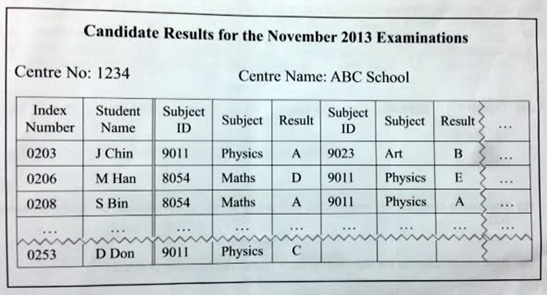
\includegraphics[width=0.5\paperwidth]{C:/Users/Admin/Desktop/Github/question_bank/LyX/static/img/9597-ALVL-2013-P2-Q2-1}
\par\end{center}

Candidates can only take examinations at one centre in a particular
session.

Currently the candidate results for each centre are stored in a separate
file. The software that produces the above report is written in a
programming language.
\begin{enumerate}
\item Describe, using an example, why this file has data redundancy.\hfill{}
{[}2{]}
\item An extra field is added to the file, but the report will not include
this new field. 

Describe the problem that will arise. \hfill{}{[}3{]}
\end{enumerate}
A normalised database solution to this problem is designed, which
has a number of tables.
\begin{enumerate}
\item[(c)]  Draw an E-R diagram that shows these tables and the relationships
between them.\hfill{} {[}5{]}
\item[(d)]  When the data are stored in a database, privacy is of great concern.

Explain why.\hfill{} {[}2{]}
\end{enumerate}
{[}SPLIT\_HERE{]}
\item \textbf{{[}ALVL/9597/2013/P2/Q3{]} }

A hash table has an index range of 1 to 900. The following pseudocode
describes an algorithm for searching the table using the hashing function
Hash. It is assumed that the key is present in the table.

\noindent %
\noindent\begin{minipage}[t]{1\columnwidth}%
\texttt{01 Index <- Hash(Key) }

\texttt{02 WHILE Table{[}Index, 1{]} <> Key }

\texttt{03 \qquad{}Index <- Index + 1 }

\texttt{04 ENDWHILE }

\texttt{05 Value <- Table{[}Index, 2{]}}%
\end{minipage}
\begin{enumerate}
\item Explain the purpose of:
\begin{enumerate}
\item line 3
\item line 5\hfill{} {[}4{]}
\end{enumerate}
\item Describe a problem that might occur with a key which, when hashed,
produces an index of 900. \hfill{}{[}2{]}
\item What modification to the algorithm is required to overcome this problem?
\hfill{}{[}3{]}
\item Explain how a new item can be added to this hash table. \hfill{}{[}4{]}
\end{enumerate}
{[}SPLIT\_HERE{]}
\item \textbf{{[}ALVL/9597/2013/P2/Q4{]} }

A software development company currently hosts its own email server.
The company is considering a replacement webmail service, using cloud
computing.
\begin{enumerate}
\item (a) State two advantages of this change.\hfill{} {[}2{]}
\item (b) State one disadvantage of this change. \hfill{}{[}1{]}
\end{enumerate}
The company is also considering other uses of the cloud. These include
collaborative activities between employees of the company and also
assistance in developing new software.
\begin{enumerate}
\item[(c)]  Describe an example of how employees of the company may use the
cloud to work collaboratively.\hfill{} {[}3{]}
\item[(d)]  Describe how the cloud can be beneficial to the company when developing
new software for a client. \hfill{}{[}4{]}
\end{enumerate}
{[}SPLIT\_HERE{]}
\item \textbf{{[}ALVL/9597/2013/P2/Q5{]} }

Bank customers are allowed to withdraw money from their accounts at
an ATM. They cannot withdraw more than the current balance in their
account. There is a daily limit on the amount that can be withdrawn.
In some circumstances a charge is made for the transaction. The rules
are:
\begin{itemize}
\item the transaction is rejected if the withdrawal amount requested is
greater than the current balance 
\item the transaction is rejected if the withdrawal amount exceeds the daily
limit 
\item if the current balance before the transaction is carried out is less
than 50 dollars then any successful transaction incurs a fixed charge
\end{itemize}
\begin{enumerate}
\item Create a decision table showing all the possible conditions and actions.
\hfill{}{[}4{]}
\item Simplify your decision table by removing redundancies. \hfill{}{[}4{]}
\item Using your answer in (b) write a function using pseudocode. The function
returns:
\begin{itemize}
\item -1 to indicate a rejection; 
\item 0 for a charge-free successful transaction; 
\item the charge for a chargeable successful transaction.\hfill{} {[}5{]}
\end{itemize}
\item State two ways in which your answer in (c) demonstrates clarity of
code. \hfill{}{[}2{]}
\end{enumerate}
{[}SPLIT\_HERE{]}
\item \textbf{{[}ALVL/9597/2013/P2/Q6{]} }

The ASCII code for the character 'Z', expressed as a denary integer,
is 90.
\begin{enumerate}
\item Express the denary integer 90 as:
\begin{enumerate}
\item an eight-bit binary number
\item a hexadecimal number \hfill{}{[}2{]}
\end{enumerate}
\item Give two reasons why hexadecimal numbers are used in computing. \hfill{}{[}2{]}
\item State the ASCII code for 'X' in denary. Explain your answer.\hfill{}
{[}2{]}
\item Explain why the Unicode encoding system has replaced ASCII. \hfill{}{[}2{]}
\item Describe a method of storing strings of characters of variable length
in a computer. \hfill{}{[}2{]}
\end{enumerate}
{[}SPLIT\_HERE{]}
\end{enumerate}
 
\end{document}
